\begin{document}
For the first prototype of our application the idea was to learn from previously done work and reuse what worked best. Additionally we followed general design principles like Gestalt laws.

A typical visualisation technique to make complex relationships clearly understandable is a graph layout. To show data flow from a data subject to one or more data processors, a graph should work very well.
Nodes represent data subject and data processors, and the links between them show that they relate with each other in such a way, that data is shared between them.
To make this even more clear actual or imaginary data packets can be visualised as moving particles between the nodes.
This feature makes it possible to give the visualisation a sense of directional flow.
\begin{figure}
    \centering
    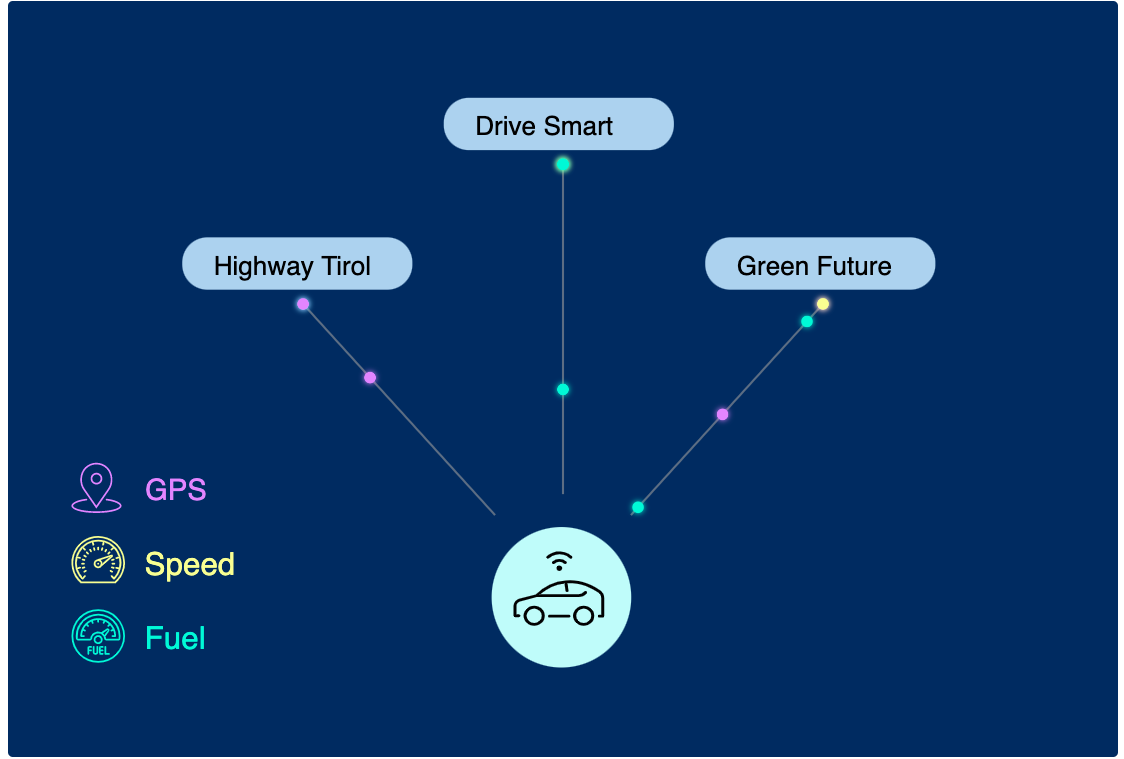
\includegraphics[width=\linewidth]{first-prototype}    \caption{The first prototype of the general overview}
    \label{fig:prototype}
\end{figure}

Since the whole application is built around giving the user a sense of control over his sharing activities, the user as a data subject stands in the center of the visualisation with the connected data processors distributed around in a circle.
Data processors, called campaigns in the CampaNeo environment, are represented by a rounded rectangle and campaign name. The round particles representing data packets flowing between user and campaign. They are color-coded to give additional information on the type of data that is sent.
The meaning of the different colors are encoded in a legend on the side of the screen. Here words are paired with unambiguous symbols to make the legend easier and faster to read.
On the whole the visualisation should enable users to see at one glance what kind of data they are sharing and at what rate.

With that we have now completely satisfied the defined needs of our application.
The user can now find out with whom he shares what data and approximately at what rate.
But in case more information should be requested, it is possible to click a certain data flow in the visualisation to get a more detailed view of the data stream.
Here we rely on a time series visualisation and give additional information about the sensor that retrieved the data and the companies that the data processor shares the data with.

The more detailed information is served just upon investigation through interaction with the visualisation as displaying everything on screen at the same time would overload the initial rendering far too much.
\end{document}
